En la figura \ref{fig:modeloProyecto} se muestra la estructura de información que manejará el sistema para registrar proyectos y los colaboradores de la organización.

\begin{figure}[htbp!]
	\begin{center}
		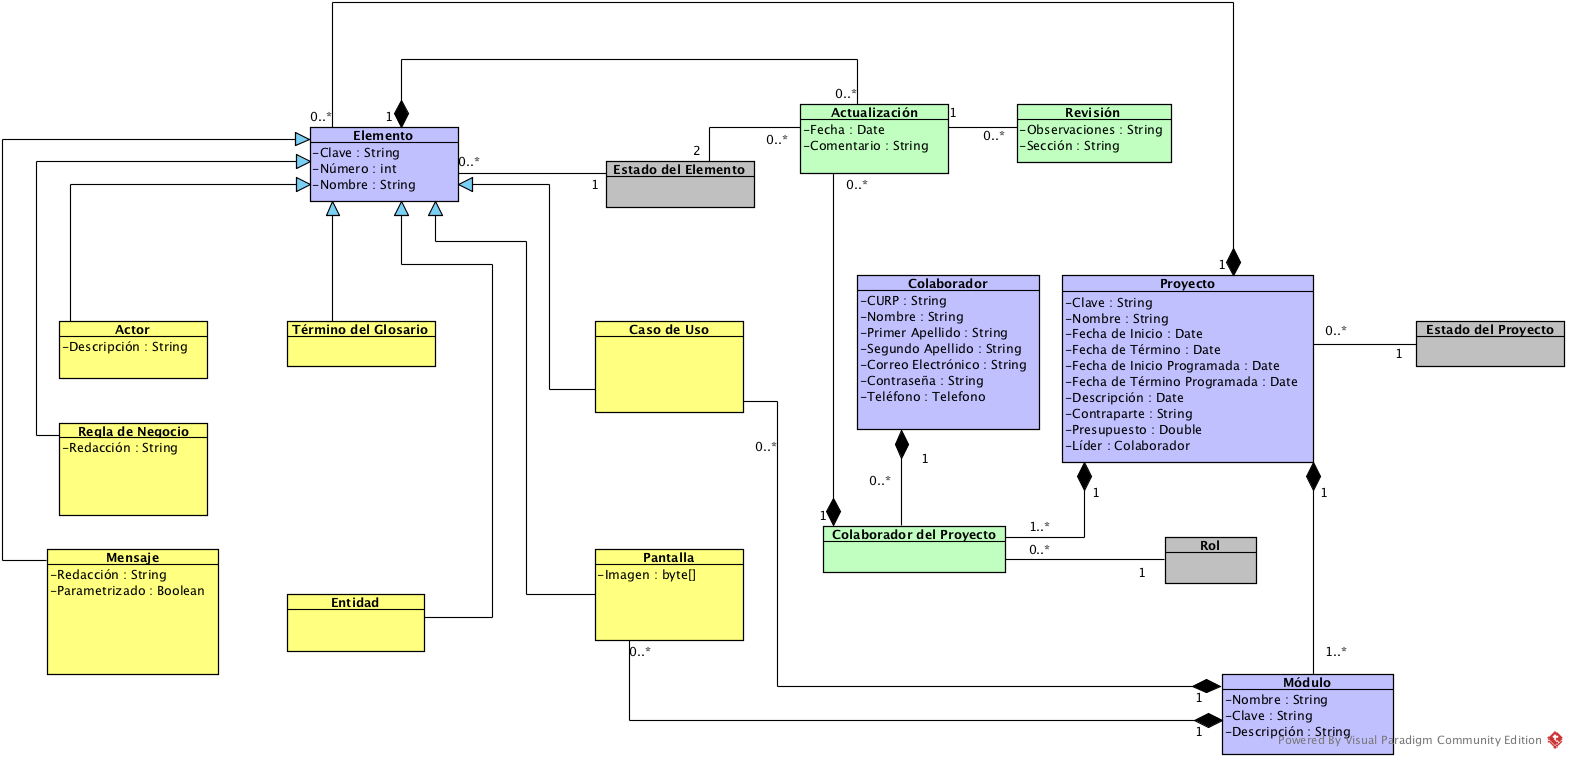
\includegraphics[angle=0,width=.95\textwidth]{images/modeloProyecto}
		\caption{Modelo conceptual de proyectos}
		\label{fig:modeloProyecto}
	\end{center}
\end{figure}

\begin{BusinessEntity}{elementoEntidad}{Elemento}
	\Battr{claveElemento}{Clave: }{Clave que permitirá distinguir el tipo de Elemento. Es una palabra corta y este dato es \hyperlink{tRequerido}{requerido} {\em (no se puede omitir)}. }
		
	\Battr{numeroElemento}{Número: }{Número del Elemento del tipo denido por la Clave. Es un valor numérico entero y este dato es \hyperlink{tRequerido}{requerido} {\em (no se puede omitir)}.}
		
	\Battr{nombreElemento}{Nombre: }{Nombre que identificará al Elemento. Es una frase o enunciado y este dato es \hyperlink{tRequerido}{requerido} {\em (no se puede omitir)}.}
\end{BusinessEntity}

\subsubsection{Relaciones}
\begin{BusinessFact}{pantallaRelElemento}{Pantalla}
	\BRitem{\textbf{Descripción: }}{Pantalla es un tipo de Elemento.}
	\BRitem{\textbf{Tipo: }}{\relHerencia}
\end{BusinessFact}

\begin{BusinessFact}{actorRelElemento}{Actor}
	\BRitem{\textbf{Descripción: }}{Actor es un tipo de Elemento.}
	\BRitem{\textbf{Tipo: }}{\relHerencia}
\end{BusinessFact}

\begin{BusinessFact}{BrRelElemento}{Reglas de Negocio}
	\BRitem{\textbf{Descripción: }}{Regla de Negocio es un tipo de Elemento.}
	\BRitem{\textbf{Tipo: }}{\relHerencia}
\end{BusinessFact}

\begin{BusinessFact}{MensajeRelElemento}{Mensaje}
	\BRitem{\textbf{Descripción: }}{Mensaje es un tipo de Elemento.}
	\BRitem{\textbf{Tipo: }}{\relHerencia}
\end{BusinessFact}

\begin{BusinessFact}{terminoRelElemento}{Término (Glosario)}
	\BRitem{\textbf{Descripción: }}{Término (Glosario) es un tipo de Elemento.}
	\BRitem{\textbf{Tipo: }}{\relHerencia}
\end{BusinessFact}

\begin{BusinessFact}{entidadRelElemento}{Entidad}
	\BRitem{\textbf{Descripción: }}{Entidad es un tipo de Elemento.}
	\BRitem{\textbf{Tipo: }}{\relHerencia}
\end{BusinessFact}

\begin{BusinessFact}{CURelElemento}{Caso de Uso}
	\BRitem{\textbf{Descripción: }}{Caso de Uso es un tipo de Elemento.}
	\BRitem{\textbf{Tipo: }}{\relHerencia}
\end{BusinessFact}

\begin{BusinessFact}{entidadRelElemento}{Entidad}
	\BRitem{\textbf{Descripción: }}{Entidad es un tipo de Elemento.}
	\BRitem{\textbf{Tipo: }}{\relHerencia}
\end{BusinessFact}

\begin{BusinessFact}{actualizacionRelElemento}{Actualización}
	\BRitem{\textbf{Descripción: }}{Un elemento ha pasado por un conjunto de actualizaciones.}
	\BRitem{\textbf{Tipo: }}{\relComposicion}
	\BRitem{\textbf{Cardinalidad: }}{Uno a muchos}
\end{BusinessFact}

\begin{BusinessFact}{estadoRelElemento}{Estado del Elemento}
	\BRitem{\textbf{Descripción: }}{Un Elemento se encuentra en un Estado.}
	\BRitem{\textbf{Tipo: }}{\relAsociacion}
	\BRitem{\textbf{Cardinalidad: }}{Muchos a uno}
\end{BusinessFact}

\begin{BusinessFact}{proyectoRelElemento}{Proyecto}
	\BRitem{\textbf{Descripción: }}{Un Proyecto se compone de elementos.}
	\BRitem{\textbf{Tipo: }}{\relComposicion}
	\BRitem{\textbf{Cardinalidad: }}{Muchos a uno}
\end{BusinessFact}

\begin{BusinessFact}{valorParamPasoRelElemento}{Valor Parámetro en Paso}
	\BRitem{\textbf{Descripción: }}{Un Elemento puede ser el valor de algún parámetro en un paso de la Trayectoria.}
	\BRitem{\textbf{Tipo: }}{\relAsociacion}
	\BRitem{\textbf{Cardinalidad: }}{Uno a muchos}
\end{BusinessFact}

\begin{BusinessFact}{valorParamMensajeRelElemento}{Valor Parámetro en Mensaje}
	\BRitem{\textbf{Descripción: }}{Un Elemento puede ser el valor de algún parámetro en un Mensaje.}
	\BRitem{\textbf{Tipo: }}{\relAsociacion}
	\BRitem{\textbf{Cardinalidad: }}{Uno a muchos}
\end{BusinessFact}

\begin{BusinessFact}{valorParamBRRelElemento}{Valor Parámetro en Regla de Negocio}
	\BRitem{\textbf{Descripción: }}{Un Elemento puede ser el valor de algún parámetro en una Regla de Negocio.}
	\BRitem{\textbf{Tipo: }}{\relAsociacion}
	\BRitem{\textbf{Cardinalidad: }}{Uno a muchos}
\end{BusinessFact}

\begin{BusinessEntity}{proyectoEntidad}{Proyecto}
	\Battr{claveProyecto}{Clave: }{Palabra que permitirá distinguir al proyecto, regularmente es la sigla del nombre. Es una palabra corta y este dato es \hyperlink{tRequerido}{requerido} {\em (no se puede omitir)}. Este atributo debe de contener como máximo 10 caracteres. Caracteres admitidos: [A-Z] $|$ [0-9]}
		
	\Battr{nombreProyecto}{Nombre: }{Nombre que identificará al proyecto. Es una frase o enunciado y este dato es \hyperlink{tRequerido}{requerido} {\em (no se puede omitir)}. Este atributo debe de contener como máximo 50 caracteres. Caracteres admitidos: [A-Z] $|$ [a-z] $|$ [á-é-í-ó-ú] $|$ []}
	
	\Battr{fechaIProyecto}{Fecha de Inicio: }{Fecha en que se arranca el proyecto. Especifica una \hyperlink{tFecha}{fecha} y este dato es \hyperlink{tOpcional}{opcional} {\em (se puede omitir)}.}
	
	\Battr{fechaFinProyecto}{Fecha de termino: }{Fecha en la que concluye el proyecto. Especifica una \hyperlink{tFecha}{fecha} y este dato es \hyperlink{tOpcional}{opcional} {\em (se puede omitir)}.}
	
	\Battr{fechaIPProyecto}{Fecha de inicio programada: }{Fecha en que se desea arrancar el proyecto. Especifica una \hyperlink{tFecha}{fecha} y este dato es \hyperlink{tRequerido}{requerido} {\em (no se puede omitir)}.}
	
	\Battr{fechaFinPProyecto}{Fecha de termino programada: }{Fecha en que se desea finalizar el proyecto. Especifica una \hyperlink{tFecha}{fecha} y este dato es \hyperlink{tRequerido}{requerido} {\em (no se puede omitir)}.}
	
	\Battr{descripcionProyecto}{Descripción: }{Párrafo que contiene las características generales del proyecto que se comenzará. Descrita en uno o más párrafos y este dato es \hyperlink{tRequerido}{requerido} {\em (no se puede omitir)}. Este atributo debe de contener como máximo 1000 caracteres. Caracteres admitidos: [A-Z] $|$ [a-z] $|$ [0-9] $|$ [  ] $|$ [-] $|$ [,] $|$ [á-é-í-ó-ú]}
	
	\Battr{liderProyecto}{Líder: }{Nombre y apellidos del líder del proyecto. Es una frase o enunciado y este dato es \hyperlink{tRequerido}{requerido} {\em (no se puede omitir)}.}
	
	\Battr{contraparteProyecto}{Contraparte: }{Es el cliente del proyecto. Es una frase o enunciado y este dato es \hyperlink{tRequerido}{requerido} {\em (no se puede omitir)}.Este atributo debe de contener como máximo 100 caracteres. Caracteres admitidos: [A-Z] $|$ [a-z] $|$ [0-9] $|$ [  ] $|$ [-] $|$ [,] $|$ [á-ú]}
	
	\Battr{presupuestoProyecto}{Presupuesto: }{Es el monto calculado del costo del proyecto. Es un valor numérico flotante y este dato es \hyperlink{tOpcional}{opcional} {\em (se puede omitir)}.}
\end{BusinessEntity}

\subsubsection{Relaciones}
\begin{BusinessFact}{elementoRelProyecto}{Elemento}
	\BRitem{\textbf{Descripción: }}{Un proyecto puede tener varios Elementos asociados como reglas de negocio, mensajes, entidades y actores.}
	\BRitem{\textbf{Tipo: }}{\relComposicion}
	\BRitem{\textbf{Cardinalidad: }}{Uno a muchos}
\end{BusinessFact}

\begin{BusinessFact}{estadoRelProyecto}{Estado del Proyecto}
	\BRitem{\textbf{Descripción: }}{Un proyecto tiene un Estado del Proyecto.}
	\BRitem{\textbf{Tipo: }}{\relAsociacion}
	\BRitem{\textbf{Cardinalidad: }}{Muchos a uno}
\end{BusinessFact}

\begin{BusinessFact}{colaboradorRelProyecto}{Colaborador del Proyecto}
	\BRitem{\textbf{Descripción: }}{Un proyecto tiene uno o varios Colaboradores del Proyecto.}
	\BRitem{\textbf{Tipo: }}{\relComposicion}
	\BRitem{\textbf{Cardinalidad: }}{Uno a muchos}
\end{BusinessFact}

\begin{BusinessFact}{moduloRelProyecto}{Módulo}
	\BRitem{\textbf{Descripción: }}{Un proyecto tiene uno o varios Módulos donde se organizarán los casos de uso y las pantallas.}
	\BRitem{\textbf{Tipo: }}{\relComposicion}
	\BRitem{\textbf{Cardinalidad: }}{Uno a muchos}
\end{BusinessFact}
\begin{BusinessEntity}{colaboradorEntidad}{Colaborador}

	\Battr{curpColaborador}{CURP}{Clave Única de Registro. Es una palabra corta y este dato es \hyperlink{tRequerido}{requerido} ({\em no se puede omitir}). Este atributo debe de contener exactamente 18 caracteres. Caracteres admitidos: [A-Z] $|$ [0-9]}
		
	\Battr{nombreColaborador}{NOMBRE: }{Nombre o nombres de pila del colaborador. Es una frase o enunciado y este dato es \hyperlink{tRequerido}{requerido} ({\em no se puede omitir}).}
		
		\Battr{pApellidoColaborador}{Primer Apellido: }{Es el primer apellido del colaborador. Es una frase o enunciado y este dato es \hyperlink{tRequerido}{requerido} ({\em no se puede omitir}).}
		
		\Battr{sApellidoColaborador}{Segundo Apellido: }{Es el segundo apellido del colaborador. Es una frase o enunciado y este dato es \hyperlink{tRequerido}{requerido} ({\em no se puede omitir}).}
		
		\Battr{correoColaborador}{Correo Electrónico: }{Es un identificador para que el usuario inicie sesión. Es una palabra corta y este dato es \hyperlink{tRequerido}{requerido} ({\em no se puede omitir}). Este atributo debe contener a lo más 50 caracteres. Es una cadena de caracteres con formato xxx@yyy.com o xxx@yyy.com.mx}
		
		\Battr{passColaborador}{Contraseña: }{Es una clave que sirve para autenticarse la cual sirve como un mecanismo de seguridad. Es una frase o enunciado y este dato es \hyperlink{tRequerido}{requerido} ({\em no se puede omitir}).}
		
		\Battr{telefonoColaborador}{Teléfono: }{Es una secuencia de dígitos que representan un número telefónico. Es un valor numérico y este dato es \hyperlink{tRequerido}{requerido} ({\em no se puede omitir}). }
\end{BusinessEntity}

\subsubsection{Relaciones}

\begin{BusinessFact}{proyectoRelColaborador}{Colaborador del Proyecto}
	\BRitem{\textbf{Descripción: }}{Un colaborador puede participar en varios proyectos}
	\BRitem{\textbf{Tipo: }}{\relAsociacion}
	\BRitem{\textbf{Cardinalidad: }}{Uno a muchos}
\end{BusinessFact}
\begin{BusinessEntity}{proyectoColEntidad}{Colaborador de Proyecto}
	\item Esta entidad es auxiliar. Sirve para corresponder el proyecto y sus colaboradores.
\end{BusinessEntity}

\subsubsection{Relaciones}
\begin{BusinessFact}{rolRelColProyecto}{Rol}
	\BRitem{\textbf{Descripción: }}{Un colaborador tiene un Rol que define si es un analista o un líder de análisis.}
	\BRitem{\textbf{Tipo: }}{\relAsociacion}
	\BRitem{\textbf{Cardinalidad: }}{Muchos a uno}
\end{BusinessFact}

\begin{BusinessFact}{actualizacionRelColProyecto}{Actualización}
	\BRitem{\textbf{Descripción: }}{Cuando un colaborador realiza cambios en los elementos se guardan las Actualizaciones.}
	\BRitem{\textbf{Tipo: }}{\relComposicion}
	\BRitem{\textbf{Cardinalidad: }}{Uno a muchos}
\end{BusinessFact}
\begin{BusinessEntity}{moduloEntidad}{Módulo}
	\Battr{claveModulo}{Clave: }{Palabra que permitirá distinguir al módulo, generalmente es la abreviación del nombre del módulo. Es una palabra corta y este dato es \hyperlink{tRequerido}{requerido} {\em (no se puede omitir)}. }
		
	\Battr{nombreModulo}{Nombre: }{Palabra que sirve para identificar el módulo. Es una palabra corta y este dato es \hyperlink{tRequerido}{requerido} {\em (no se puede omitir)}.}
	
	\Battr{descripcionModulo}{Descripción: }{Párrafo que contiene las características generales módulo. Descrita en uno o más párrafos y este dato es \hyperlink{tRequerido}{requerido} {\em (no se puede omitir)}.}
\end{BusinessEntity}

\subsubsection{Relaciones}
\begin{BusinessFact}{CURelModulo}{Caso de uso}
	\BRitem{\textbf{Descripción: }}{Un módulo puede contiener varios Casos de uso.}
	\BRitem{\textbf{Tipo: }}{\relComposicion}
	\BRitem{\textbf{Cardinalidad: }}{Uno a muchos}
\end{BusinessFact}

\begin{BusinessFact}{pantallaRelModulo}{Pantalla}
	\BRitem{\textbf{Descripción: }}{Un módulo puede contener varias Pantallas.}
	\BRitem{\textbf{Tipo: }}{\relComposicion}
	\BRitem{\textbf{Cardinalidad: }}{Uno a muchos}
\end{BusinessFact}
\begin{BusinessEntity}{actualizacionEntidad}{Actualización}
	
	\Battr{fechaActualizacion}{Fecha: }{Fecha en que se realiza la actualización. Especifica una \hyperlink{tFecha}{fecha} y este dato es \hyperlink{tRequerido}{requerido} {\em (no se puede omitir)}.}
	
	\Battr{comentarioActualizacion}{Comentario: }{Descripción de los cambios realizados en los elementos. Es una frase o enunciado y este dato es \hyperlink{tRequerido}{requerido} {\em (no se puede omitir)}.}
\end{BusinessEntity}

\subsubsection{Relaciones}
\begin{BusinessFact}{revisionRelActualizacion}{Revisión}
	\BRitem{\textbf{Descripción: }}{Un analista debe hacer revisiones de las actualizaciones de los elementos.}
	\BRitem{\textbf{Tipo: }}{\relAsociacion}
	\BRitem{\textbf{Cardinalidad: }}{Uno a muchos}
\end{BusinessFact}

\begin{BusinessFact}{estadoElemRelActualizacion}{Estado del Elemento}
	\BRitem{\textbf{Descripción: }}{Una actualización debe indicar de que a que estado ha cambiado el elemento.}
	\BRitem{\textbf{Tipo: }}{\relAsociacion}
	\BRitem{\textbf{Cardinalidad: }}{Muchos a uno}
\end{BusinessFact}
\begin{BusinessEntity}{revisionEntidad}{Revisión}
	
	\Battr{observacionRevision}{Observaciones: }{Descripción de las correcciones que necesita el caso de uso. Descrita en uno o más párrafos y este dato es \hyperlink{tRequerido}{requerido} {\em (no se puede omitir)}.}
	
	\Battr{seccionRevision}{Sección: }{Es la sección sobre la que se hacen las correcciones. Es una frase o enunciado y este dato es \hyperlink{tRequerido}{requerido} {\em (no se puede omitir)}.}
\end{BusinessEntity}

\subsubsection{Relaciones}
\begin{BusinessFact}{actualizacionRelRevision}{Actualización}
	\BRitem{\textbf{Descripción: }}{El analista realiza una revisión de la Actualización.}
	\BRitem{\textbf{Tipo: }}{\relAsociacion}
	\BRitem{\textbf{Cardinalidad: }}{Muchos a uno}
\end{BusinessFact}